% Sample file on how to use subfiles.
\documentclass[ExampleMasters.tex]{subfiles}

\begin{document}
\clearpage
{\pagestyle{empty}\cleardoublepage}%
\chapter{Discussion}
\label{chap:discussion}

%\section{Results from bench testing}
%\label{sec:results_bench}

%\begin{itemize}%
%	\item lessons-learned?
%	\item adaptation for future projects
%	\item what was taken over for further tests? 
%	\item what couldnt be simultaed?
%\end{itemize}

\section{Results from processing time evaluation}
\label{sec:results_processing_time}

Figure \ref{fig:step_input} shows the requested angle, target angle and actual angle of the dolly's front axle over time. As described in section \ref{sec:measuring_delay} the requested angle is a step input, in this case of 5 degree.\\
\begin{figure*}[!hbt]
	\centering
	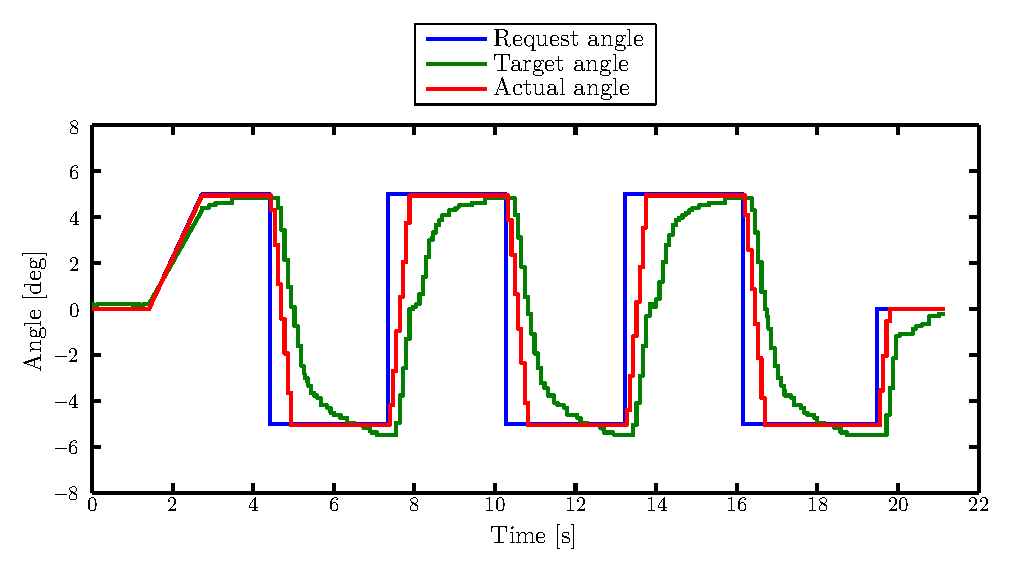
\includegraphics[width=1\linewidth]{figures/lifted_front_5deg}
	\caption{Step input 5 degree}
	
	\label{fig:step_input}
\end{figure*}
The target angle's slope is constant and lower than the slope of the request angle. The actual angle has approximately the same slope as the target angle, but it is delayed. The actual angle tends to overshoot the requested angle for falling slopes. Furthermore the slope of the actual angle is reduced when the actual angle almost reached the request. There is also a saddle point around an angle of 0 degree for rising slopes of the actual angle.          
The delays over the different request angle step inputs were plotted and a linear regression was made to deduct the actual delay for small changes of the request angle. This delay is the relevant delay, since in real driving situations the requested angle is never a step input but rather changes only slowly. The delay over the step inputs together with the linear regression is shown in figure \ref{fig:delay_testing_lin_interpolation}.    

\begin{figure*}[!hbt]
	\centering
	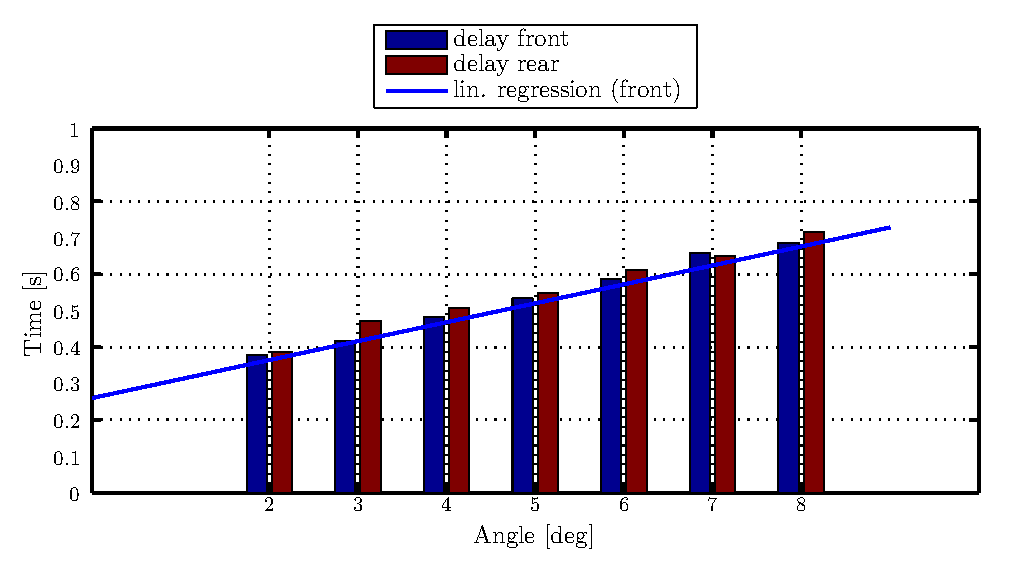
\includegraphics[width=1\linewidth]{figures/delay_testing_lin_interpolation}
	\caption{Rise time from send out request to achieve a certain steering angle on the dolly.}
	\label{fig:delay_testing_lin_interpolation}
\end{figure*}
The deducted delay is 0.26s for the front axle and 0.3s for the rear axle.
During plot analysis of preliminary results it was discussed, whether it would be possible to by-pass the occuring delay by feeding a ramp-input instead of a step-input into the \gls{ETS}. It was assumed that there is a low-pass filter in place which would not affect ramp inputs. Subsequent tests with ramp inputs with varying slopes and amplitudes showed that it was indeed possible to eliminate the low-pass filter leading to no delay between the target angle and the request angle. Examples of the ramp inputs with different rates can be seen in the figures \ref{fig:rate_limiter1}, \ref{fig:rate_limiter2} and \ref{fig:rate_limiter3}.\\
\begin{figure*}[!htb]
	\centering
	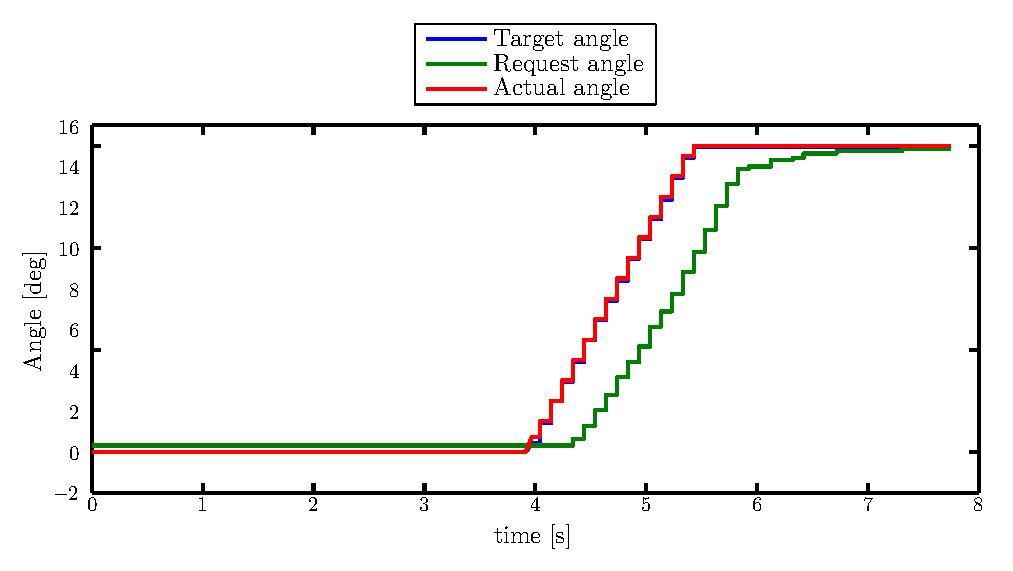
\includegraphics[width=1\linewidth]{figures/rate_limiter1}
	\caption{Ramp input rate 0.01}
	
	\label{fig:rate_limiter1}
\end{figure*}
\begin{figure*}[!hbt]
	\centering
	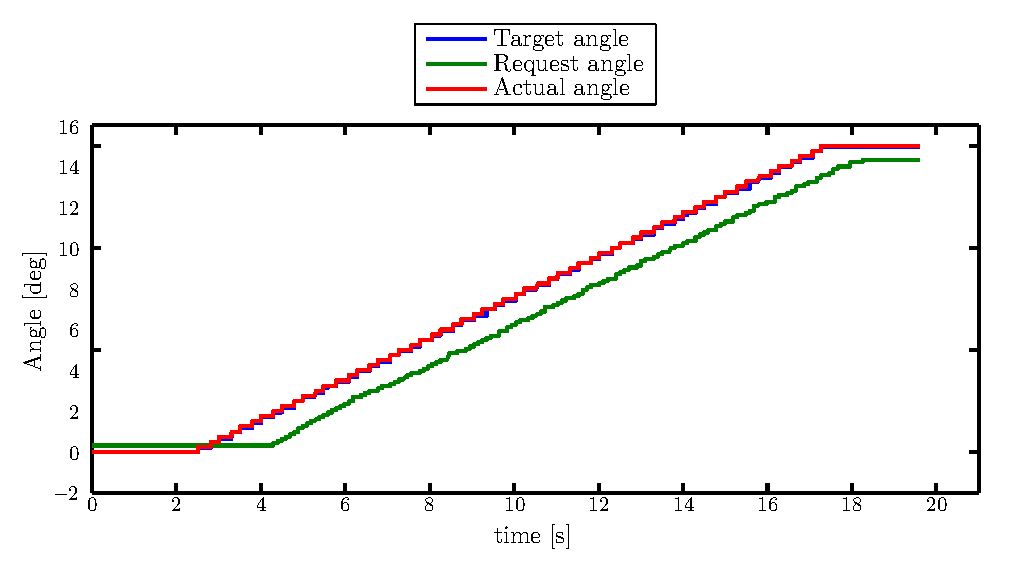
\includegraphics[width=1\linewidth]{figures/rate_limiter2}
	\caption{Ramp input rate 0.001}
	
	\label{fig:rate_limiter2}
\end{figure*}
\begin{figure*}[!hbt]
	\centering
	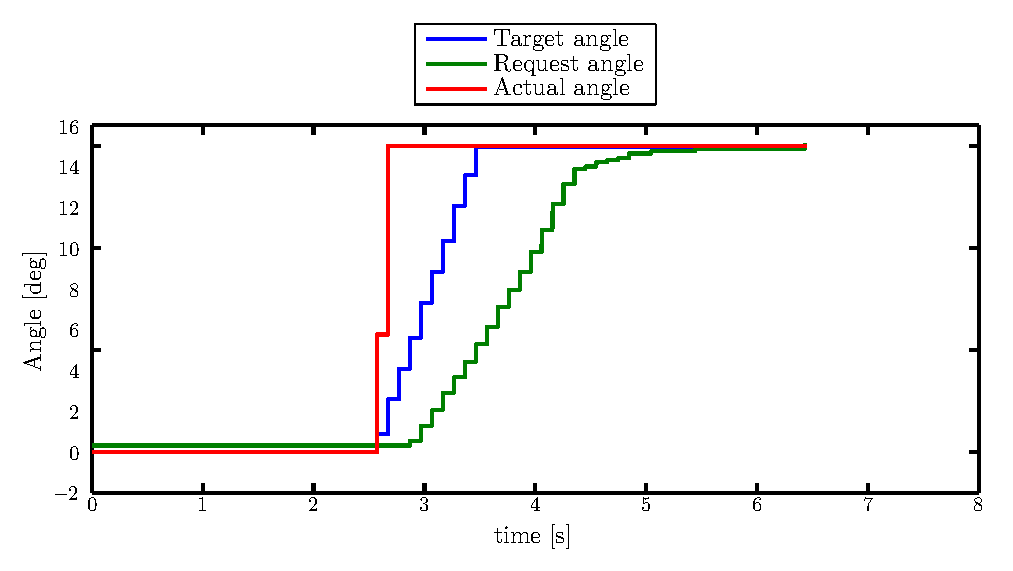
\includegraphics[width=1\linewidth]{figures/rate_limiter3}
	\caption{Ramp input rate 0.1}
	
	\label{fig:rate_limiter3}
\end{figure*}

With a rate of 0.01 the request angle and target angle align. They also align at a rate of 0.001 but for that case their slope is much lower, so it takes a insufficient long time to reach the indented angle. For a rate of 0.1 the signals of the request angle and the target angle don't align anymore. For rates higher than 0.3, the \gls{ETS}-system switches to alarm mode, because the request angle changes to fast, so the signal is implausible for the system.   


Comparing figure \ref{fig:rate_limiter1} and figure \ref{fig:rate_limiter3} indicates that it is not possible to get any faster change with a ramp input than with the request of a step input. It thus can be concluded that the maximum steering rate of $5 ^\circ /s$ can not be circumvented.


%\section{Results from in vehicle testing}
%\label{sec:results_vehicle_testing}




%\begin{itemize}
%	\item CAN-analysis
%%	\item robustness?
%	\item reliability of safety features
%\end{itemize}


\section{Results from hardware-in-the-loop testing}

Figure \ref{fig:HIL002_front} shows the measurements of the ETS-CAN of the front axle of the dolly for the low-speed maneuver described in section \ref{sec:HIL}.\\

\begin{figure*}[!htb]
	\centering
	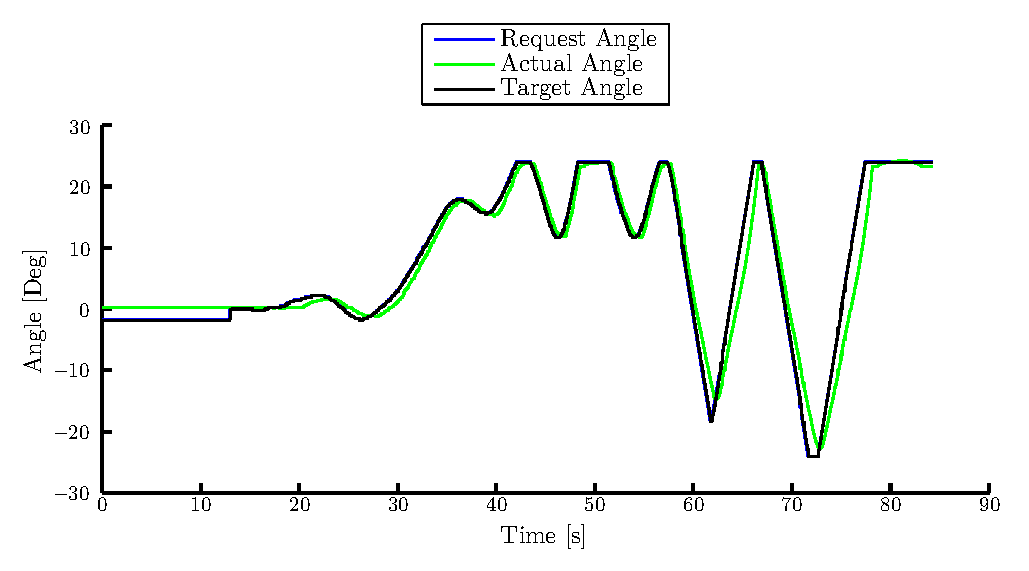
\includegraphics[width=1\linewidth]{figures/HIL002_front}
	\caption{HIL-test low-speed front axle}
	
	\label{fig:HIL002_front}
\end{figure*}

The request angle is the angle that was requested from the controller and then sent from the sSimulation-PC to the \gls{MABII}. The target angle is the angle that was calculated by the \gls{ETS}-\gls{ECU} and sent as a request to the actuators of the dolly. The actual angle is the angle that the sensors on the dolly's wheels measured and which is the articulation of the dolly's wheel on the ground.
Figure \ref{fig:HIL002_rear} shows the same measurements for the rear axle.

\begin{figure*}[!htb]
	\centering
	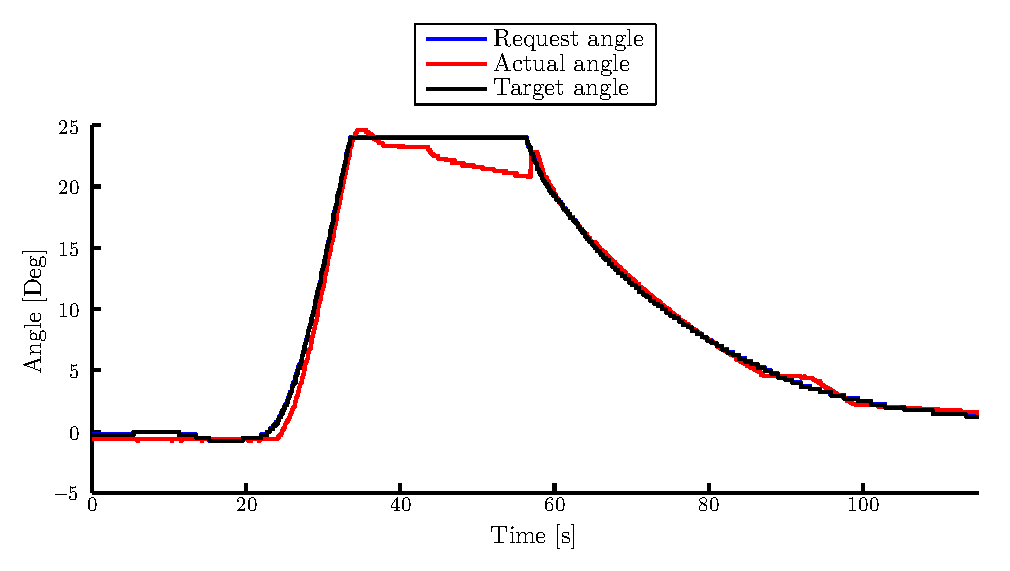
\includegraphics[width=1\linewidth]{figures/HIL002_rear}
	\caption{HIL-test low-speed rear axle}
	
	\label{fig:HIL002_rear}
\end{figure*}
Since the same requested angle for front and rear is the same, below only the front axle is looked upon. Both axles show a very similar behaviour and thus only considering one is justifiable.
Figure \ref{fig:HIL002_front_closeup} shows an extraction of the measurements of the front axle. 
\begin{figure*}[!htb]
	\centering
	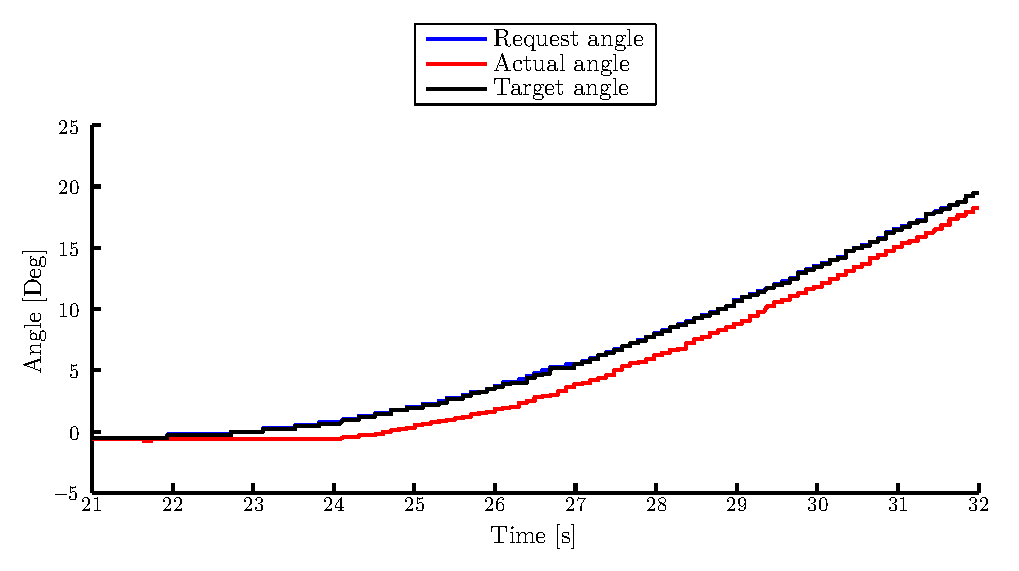
\includegraphics[width=1\linewidth]{figures/HIL002_front_closeup}
	\caption{Details of HIL-test low-speed front axle}
	
	\label{fig:HIL002_front_closeup}
\end{figure*} \\
As already mentioned in section \ref{sec:measuring_delay} there is a delay between the angle requested of the \gls{ETS}-\gls{ECU} and the actual angle of the wheels. This can very distinctifvly be seen in this plot. In comparison to this, the delay between the angle request that is sent from the \gls{MABII} to the \gls{CAN} and the target angle that is sent from the \gls{ETS}-\gls{ECU} to the actuators is very small and can therefore be neglected.\\

To get an impression of the overall results of the \gls{HIL}-test, figure \ref{fig:HIL002_complete} shows the measurements conducted on the simulation-PC and the measurements done in ControllDesk in the same plot. 
\begin{figure*}[!htb]
	\centering
	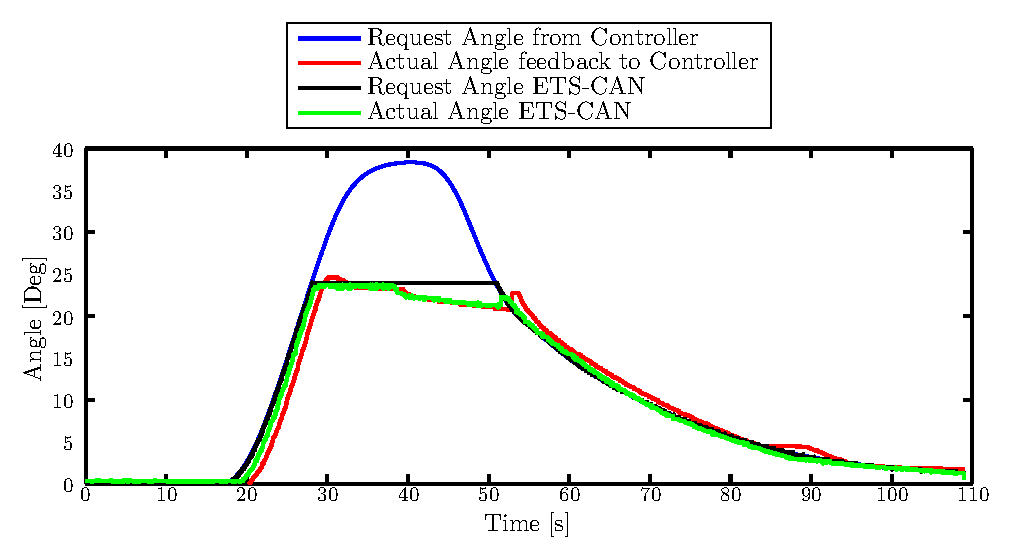
\includegraphics[width=1\linewidth]{figures/HIL006_alles}
	\caption{HIL-test front axle measurements from VTM and ETS-CAN}	
	\label{fig:HIL002_complete}
\end{figure*}

For one thing the plot shows the limitation of the angle that is requested from the controller by the supervisor block described in section \ref{sec:warning_system}. For another thing it shows that there is a relatively high delay between the signal of the actual angle of the dolly from the \gls{ETS}-\gls{CAN} and the signal that is feedback to the simulation-PC. This is most likely caused by the use of the serial interface to transmit the signal from the CAN to the simulation-PC. \\
To get a more detailed view of this delay as well as the limitation of the request angle figure \ref{fig:HIL002_complete_details} shows a extraction of figure \ref{fig:HIL002_complete}.   

\begin{figure*}[!htb]
	\centering
	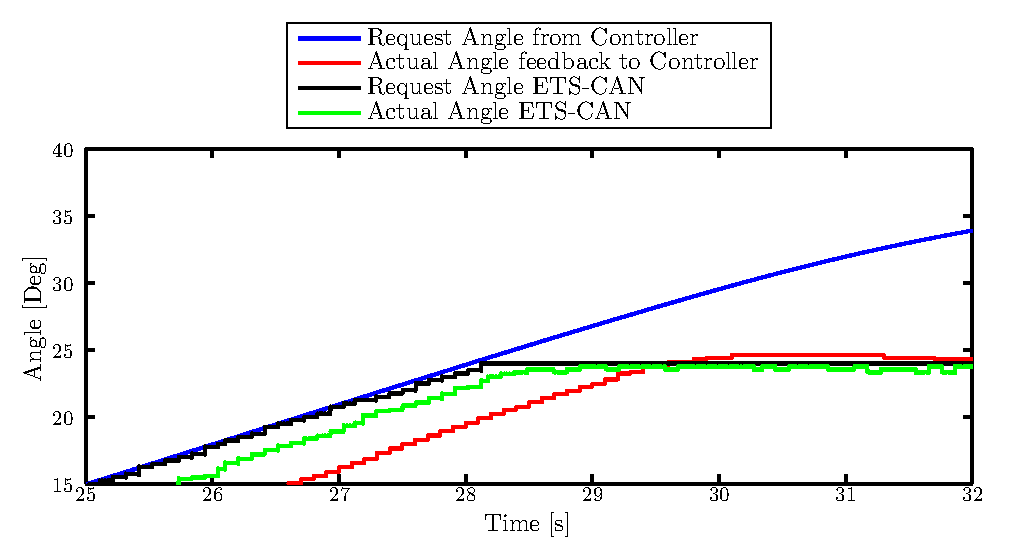
\includegraphics[width=1\linewidth]{figures/HIL006_alles_details}
	\caption{Details of \gls{HIL}-test front axle measurements from \gls{VTM} and \gls{ETS}-\gls{CAN}}
	
	\label{fig:HIL002_complete_details}
\end{figure*}


The tested controller was evaluated in \gls{HIL} testing as well as in pure simulation in \gls{VTM}. The two resulting curves of the vehicles path can be seen in figures \ref{fig:xy_HIL} for the \gls{HIL}-testing and \ref{fig:xy_VTM} for the pure \gls{VTM}-simulation of the same maneuver respectively. For easier comparison figure \ref{fig:xy_HIL_and_VTM} depicts the pathes for both environments. The steering reacts a bit slower for the \gls{HIL}-tests, but overall the paths are very similiar. The actual performance of the algorithm and its evaluation is not part of this thesis, but it was the to have an as similar matching between simulation and \gls{VTS} environment.


\begin{figure*}[!htb]
	\centering
	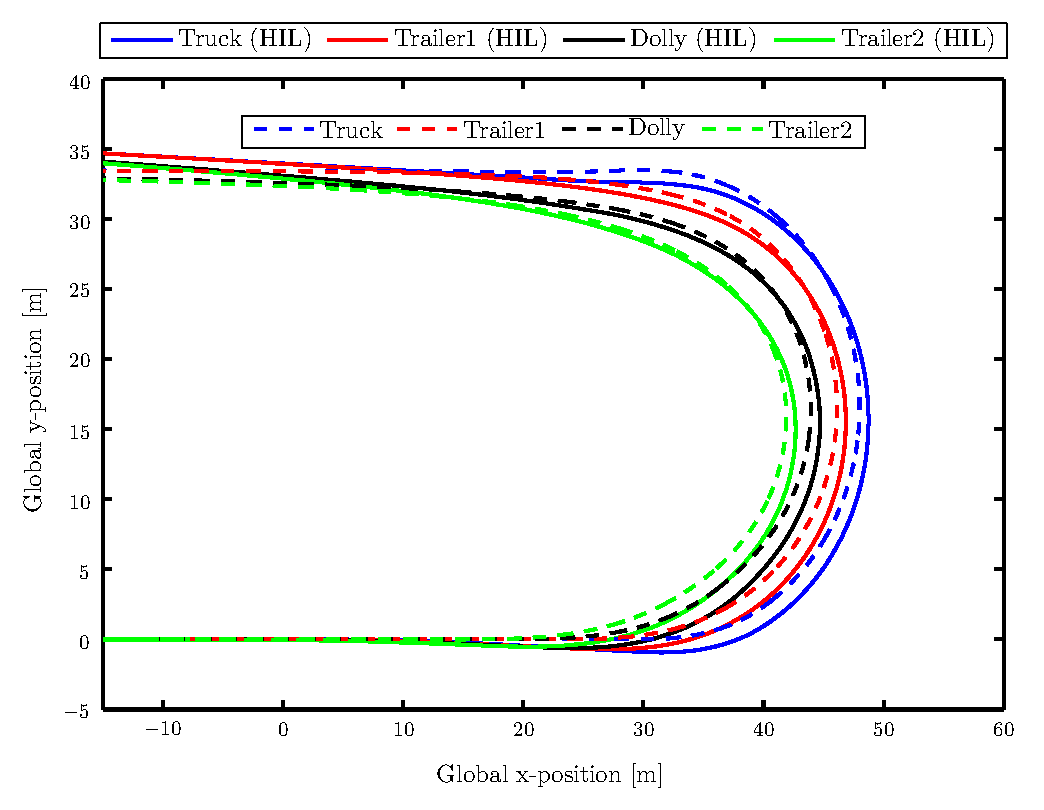
\includegraphics[width=1\linewidth]{figures/xy_HIL_and_VTM}
	\caption{Comparison between swept pathes of different units in the \gls{HCT} combination during \gls{HIL}-testing and \gls{VTM}-simulation}
	
	\label{fig:xy_HIL_and_VTM}
\end{figure*}

As can be gathered from figure \ref{fig:compare_HIL_VTS}, the error between the two environments accumulates over time. This is a consequence of slightly different paths they choose due to the dolly not really allowing steering of very small angles (-1 to 1$^\circ$). This is caused by hardware limitations and a dead-band filter which is present in the \gls{ETS}-\gls{ECU}. The end of the measuring can practically be ignored from approximately 100m of distance traveled, as this is mostly caused by different angles at which the combination exits the turn. This can be compensated for by fine-tuning the steering inputs, which was omitted for this thesis, as it was only the aim to demonstrate the general function of the controller. Fine-tuning will only be conducted once the final controller is ready and correctly implemented. 

\begin{figure*}[!htb]
	\centering
	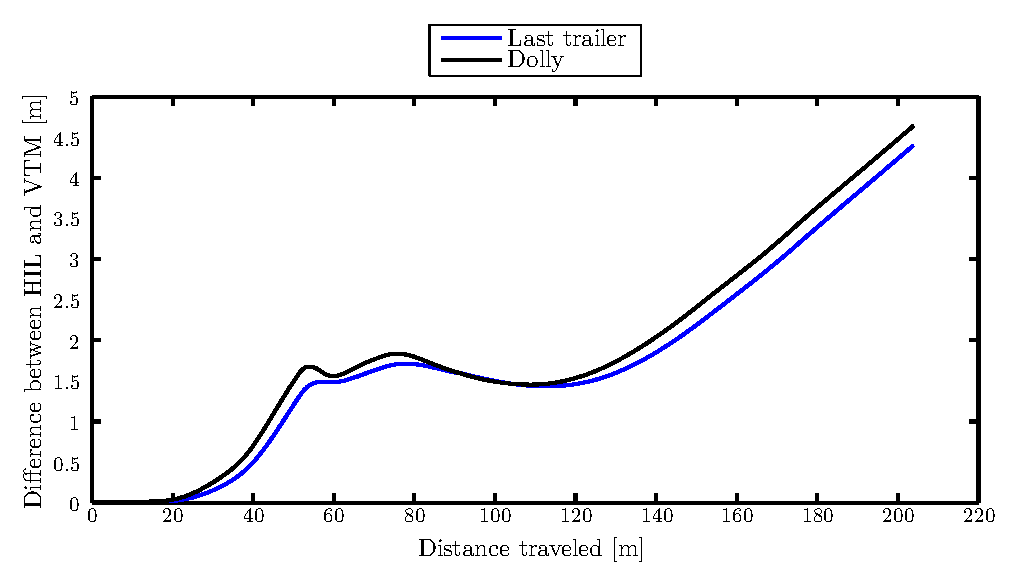
\includegraphics[width=1\linewidth]{figures/compare_HIL_VTS}
	\caption{Deviation between \gls{HIL}-testing and \gls{VTM}-simulation plotted over distance traveled during 180$^\circ$-turn}
	
	\label{fig:compare_HIL_VTS}
\end{figure*}


\end{document}
